\documentclass[
    iict, % Saisir le nom de l'institut rattaché
    il, % Saisir le nom de l'orientation
    %confidential, % Décommentez si le travail est confidentiel
]{heig-tb}

\usepackage[nooldvoltagedirection,european,americaninductors]{circuitikz}

\signature{jFriedli.svg} % Remplacer par votre propre signature vectorielle.

\makenomenclature
\makenoidxglossaries
\makeindex

\addbibresource{bibliography.bib}

\input{nomenclature}
\input{acronyms}
\input{glossary}
% Auteur du document (étudiant-e) en projet de Bachelor
\author{Jonathan Friedli}

% Activer l'option pour l'accord du féminin dans le texte
\genre{male}

% Titre de votre travail de Bachelor
\title{Portail de quiz et drill pour examens sur ordinateur}

% Le sous titre est optionnel
\subtitle{Travail de Bachelor}

% Nom du professeur responsable
\teacher {Prof. Y. Chevallier (HEIG-VD)}

% Mettre à jour avec la date de rendu du travail
\date{\today}

% Numéro de TB
\thesis{7212}



\surroundwithmdframed{minted}

%% Début du document
\begin{document}
\selectlanguage{french}
\maketitle
\frontmatter
\clearemptydoublepage

%% Requis par les dispositions générales des travaux de Bachelor
\preamble
\authentification

%% Résumé / Résumé publiable / Version abrégée
\begin{abstract}
    % Francais
Dans le courant de l'année 2020, le professeur Yves Chevallier a réalisé une plateforme web permettant à ses élèves de réaliser des quiz interactifs. Cette plateforme a été réalisée à l'aide du framework PHP, Laravel pour le backend et du framework javascript, Vue.js pour le frontend.

Un précédent travail de Bachelor a eu pour but d'y ajouter la gestion de travaux écrits. La gestion de ces derniers n'étant pas entièrement fonctionnelle, un second travail de Bachelor a été soumis.

Dans un premier temps, ce travail apportera un refactoring du code pour porter le projet sur la version 10 de Laravel et sur la version 3 de Vue.js.

Dans un second temps, il complétera la gestion des travaux écrits comportant différents types de questions telles que des Questions à choix multiples, des questions de développement, des textes à trou, des questions de code, etc.

Finalement il aura pour but d'implémenter l'algorithme SM-2 (SuperMemo - Wikipedia) de Anki afin de permettre aux étudiants un drill avec des questions générées.

Les utilisateurs ciblés par cette plateforme sont les professeurs et étudiants de la HEIG-VD, c'est pourquoi l'authentification sera effectuée au travers du keycloak de l'école.

\asterism

\end{abstract}

%% Sommaire et tables
\clearemptydoublepage
{
    \tableofcontents
    \let\cleardoublepage\clearpage
    \listoffigures
    \let\cleardoublepage\clearpage
    \listoftables
    \let\cleardoublepage\clearpage
    \listoflistings
}

\printnomenclature
\clearemptydoublepage
\pagenumbering{arabic}

%% Contenu
\mainmatter
\chapter{Introduction}

\section{Contexte}
Dans le courant de l'année 2020, le Professeur Yves Chevallier a réalisé une plateforme web permettant à ses élèves de réaliser des quiz interactifs. Cette plateforme a été réalisée à l'aide du \emph{framework} PHP, Laravel \cite{Laravel} pour le \emph{backend} et du \emph{framework} javascript, VueJs \cite{Vuejs} pour le \emph{frontend}.

Par la suite, un travail de Bachelor a été proposé afin que cette plateforme permette aux élèves d'y effectuer des travaux écrits. Cela apporte des avantages conséquents autant pour les professeurs que pour les élèves. En effet, la plateforme permet une correction partielle du travail écrit (notamment pour les questions QCM) mais elle permet également aux élèves d'écrire du code et de le compiler. Deux choses complétement impossibles avec des tests papiers.


%%if
\section{Situation}
L'application web créée par le Professeur Yves Chevallier est \emph{open-source} et peut être trouvé à l'adresse suivante : \url{https://github.com/heig-vd-tin/heig-quiz}. Voici le dernier \href{https://github.com/heig-vd-tin/heig-quiz/commit/28fb1ac5367931f6aa986041fb992c651c9816cd}{\emph{commit}} au moment du début de mon travail.

L'ajout de travaux écrits a été en partie réalisé, mais cette partie est incomplète. Actuellement, le projet n'est pas complétement fonctionnel et la documentation contient pas mal de lacunes rendant la reprise de ce projet plus difficile que nécessaire. De plus, cette plateforme utilise d'anciennes versions de Laravel et de VueJs. Il convient donc de mettre ces technologies à jour.

\subsection{Environnements de développement}
Comme mentionné précédemment, le code source de ce projet se trouve sur un seul \emph{repository} Github \emph{open-source}. Il s'agit donc d'un \emph{mono-repository}. Il est également important de savoir que cette application a été développée dans WSL2 (\emph{Windows Subsystem for Linux v2}). Un utilisateur souhaitant contribuer au projet avec un système d'exploitation Windows se verra donc dans l'obligation d'installer WSL2.

C'est cependant une bonne chose de développer dans l'environnement WSL2 pour les utilisateurs de Windows. En effet, les installations de dépendances y sont bien plus rapides et cela permet une meilleure collaboration avec les utilisateurs d'autres systèmes d'exploitation.

\subsection{Backend}
Le \emph{backend} de cette application est une API REST. Il a été réalisée à l'aide du \emph{framework} PHP, Laravel dans sa version 8. Cette version est désormais quelque peu obsolète et il convient donc de la mettre à jour.

\subsection{Frontend}
Le \emph{frontend} de cette application a été réalisée à l'aide du \emph{framework} javascript, Vue.js dans sa version 2. Il utilise également un peu de Bootstrap et du CSS pour le style de l'application. Comme pour le \emph{backend}, le \emph{frontend} utilise des technologies qui sont désormais vieilllisantes et il serait opportun de les mettre à jour.

\subsection{Base de données}
La base de données utilisée par cette application est une base de données MySQL \cite{MySQL}. Cette dernière tourne dans un container  \cite{Docker}, ce qui offre plus de flexibilité aux utilisateurs. En effet, il n'est pas nécessaire d'installer un serveur MySQL sur sa machine pour pouvoir utiliser cette application.

\section{Cahier des charges}
Il me parait maintenant important de définir quels sont les objectifs du projet.

\subsection{Objectifs}
Les objectifs principaux de ce travail de Bachelor s'organisent autour de deux axes :

\begin{enumerate}
    \item Le remaniement du code : comme mentionné précédemment, il est important de tenir le projet et la documentation à jour afin qu'il soit le plus simple possible à reprendre et à modifier. C'est pourquoi je vais me baser sur le code existant afin de réécrire cette plateforme avec les technologies détaillées au chapitre suivant.
    \item L'ajout de l'algorithme SuperMemo d'Anki permettant ainsi aux élèves de se driller avec des quiz de révision ainsi que la finalisation de la gestion des travaux écrits. Pour rappel, l'algorithme SuperMemo permet de noter avec quelle facilité l'étudiant répond à une question. En fonction cette notation, la question reviendra plus ou moins souvent. Cela permet de tomber plus régulièrement sur des questions nous posant un problème. Dans notre cas, nous n'allons pas demander à l'élève de noter la difficulté de la question, mais nous allons nous baser sur le temps que ce dernier a mis à y répondre.
\end{enumerate}

\newpage

Voici les objectifs tels que défini dans le cahier des charges :
\subsection*{Objectifs fonctionnels}
\begin{itemize}
    \item Le projet doit avoir une documentation précise expliquant comment l'installer et le lancer
    \item Un utilisateur doit pouvoir s'identifier à la plateforme à l'aide de son compte de l'école
    \item Un professeur doit pouvoir créer et ajouter des étudiants une classe
    \item Un professeur doit pouvoir créer, via une interface, plusieurs types de questions :
          \subitem – QCM
          \subitem – Texte à trou
          \subitem – Question à développement
          \subitem – Question de code
    \item Les questions utilisent un format Markdown modifié et il doit donc y avoir une page de documentation expliquant comment créer chaque type de question.
    \item Un professeur doit pouvoir créer et gérer un quiz contenant des questions
    \item Un professeur doit pouvoir créer un travail écrit
    \item Un professeur doit pouvoir planifier un travail écrit
    \item Un travail écrit doit s'arrêter après la fin du temps imparti
    \item Un professeur doit pouvoir lancer la correction automatique des questions simples (QCM, texte à trou)
    \item Une fois, le travail écrit corrigé, un professeur doit avoir accès aux statistiques de bonne réponse des questions.
    \item Un élève doit pouvoir faire des quiz.
    \item Un étudiant doit pouvoir utiliser le mode drill du quiz
    \item Un élève doit pouvoir répondre aux questions d'un travail écrit
    \item Un élève doit pouvoir compiler son code
    \item Un élève doit pouvoir rendre son examen avant la fin du temps imparti
\end{itemize}

\subsection*{Objectifs non-fonctionnels}

\begin{itemize}
    \item L'interface doit être fluide et intuitive pour les utilisateurs
    \item L'application doit être fonctionnelle et fiable
    \item Un CI/CD doit être mis en place afin de faciliter la reprise du projet et son déploiement
    \item L'application est open source et le code est hébergé sur GitHub
    \item Les réponses d'un élève ne doivent pas pouvoir être modifiée après la fin de l'examen
    \item Les questions de l'examen ne doivent pas être modifiables après l'examen en question
    \item Les messages d'erreur doivent être clairs et compréhensibles pour l'utilisateur
\end{itemize}
%%fi

\chapter{Analyse}
Le but de cette section est d'analyser quels sont les besoins des différents utilisateurs et de trouver quelle est la meilleure manière d'y répondre. Un autre point très important de cette section est le détail des choix technologiques. Je vais donc les passer en revue et les expliquer.
\section{Besoins}

Dans un premier temps, il convient d'identifier quels seront les différents types d'utilisateurs de cette plateforme de quiz. Il y a selon moi deux types bien distincts d'utilisateurs :
\begin{itemize}
    \item Les étudiants
    \item Les professeurs
\end{itemize}

Les premiers utilisent cette plateforme afin de répondre à des quiz. La forme de ces derniers peut varier entre un simple quiz, un drill dans le but de réviser un examen ou finalement l'examen en lui-même. Ils ont donc besoin d'une interface où ils peuvent voir et choisir un quiz parmi tous ceux dont l'accès leurs est autorisé. Il doit pouvoir répondre au quiz et dans le cadre d'un examen ou d'un devoir, il doit pouvoir le rendre. Il doit également pouvoir naviguer dans le quiz.

Les professeurs quant à eux ont des besoins bien différents. Ils veulent principalement créer des quiz avec des questions de plusieurs types tels qu'un QCM, des textes à trous ou encore des questions de code. Ils doivent également pouvoir regrouper leurs étudiants en différentes classes et autoriser cette classe à répondre à certains quiz. De plus, ils peuvent créer et faire passer des examens sur cette plateforme. Dernièrement, ils ont besoin de pouvoir corriger automatiquement certaines questions comme les QCM.

Les besoins ont déjà bien été identifié et décrit par M. Stéphane Bouyiatiotis dans son rapport de TB et je vous invite donc à le consulter. Je vais, pour ma part, me concentrer sur les besoins centrés sur la partie "questionnaire de \emph{drill}".

\subsection{Drill}

Voici nos différents cas d'utilisations concernant la partie \emph{drill} de la plateforme.

% TODO changer cette histoire de temps pour le drill
\fig[H, width=14cm]{Cas d'utilisation du mode drill}{useCaseDrill.drawio}

Sur ce schéma, on constate que l'utilisation diffère drastiquement entre les deux types d'utilisateurs. Le professeur définit quelles questions pourront être dans le mode \emph{drill}. L'étudiant, quant à lui, veut choisir un sujet de question et y répondre le mieux possible. Il souhaite également que les questions auxquelles il répond de manière incorrecte ou très lente reviennent plus fréquemment que les autres.

\subsection*{Besoins liés au mode drill}
Dans ce tableau, je liste et numérote les besoins des utilisateurs.
\begin{table}[h]
    \begin{center}
        \caption{Besoins des utilisateurs \label{Besoins}}
        \begin{tabular}{|l|l|}
            \hline
            \textbf{} & \textbf{Besoins}                                                            \\
            \hline
            B1        & Choisir le sujet et le nombre de questions                                  \\
            \hline
            B2        & Choisir le temps que va durer le \emph{drill}                               \\
            \hline
            B3        & Lorsqu'on trouve une question facile, elle doit revenir moins fréquemment   \\
            \hline
            B4        & Lorsqu'on trouve une question difficile, elle doit revenir plus fréquemment \\
            \hline
            B5        & Contrôler les questions apparaissant de ce mode                             \\
            \hline
        \end{tabular}
    \end{center}
\end{table}

Une fois ces besoins identifiés, il faut les lier aux différentes fonctionnalités de notre application.

\begin{table}[h]
    \begin{center}
        \caption{Besoins des utilisateurs \label{Besoins}}
        \begin{tabular}{|l|l|l|}
            \hline
            \textbf{} & \textbf{Fonctionnalités}                                                      & \textbf{Besoins lié} \\
            \hline
            F1        & Fournir une interface permettant de personnaliser le \emph{drill}             & B1, B2               \\
            \hline
            F2        & Sélecteur pour choisir le sujet et le nombre de questions                     & B1                   \\
            \hline
            F3        & Sélecteur pour choisir le temps que va durer le \emph{drill}                  & B2                   \\
            \hline
            F4        & Récupérer un nombre défini de questions en fonction de l'utilisateur          & B5                   \\
            \hline
            F5        & Calculer la fréquence de la question en fonction du temps de réponse          & B3, B4               \\
            \hline
            F6        & Calculer la fréquence de la question en fonction de son résultat              & B3, B4               \\
            \hline
            F7        & Editer une question pour la faire apparaitre ou non dans le mode \emph{drill} & B5                   \\
            \hline
        \end{tabular}
    \end{center}
\end{table}



\section{Technologies}
Dans cette sous-section, je vais détailler les différentes technologies qui seront utilisées dans ce projet.
\subsection{Technologies présentes dans l'application}
Je vais brièvement rappeler les choix technologiques qui ont déjà été pris pour ce projet :
\begin{itemize}
    \item Pour le SGBD : MySQL.
    \item Pour le \emph{backend} : le \emph{framework} PHP, Laravel version 8.
    \item Pour le \emph{frontend} : le \emph{framework} javascript, Vue.js version 2.
    \item Pour le style de l'application : Bootstrap et CSS
    \item Pour la connexion à l'application (SSO) : Shibboleth
    \item Système de gestion de version : Github
\end{itemize}

\subsection{Choix technologiques}
Je vais maintenant expliquer et détailler chaque technologie qui sera utilisée au cours de ce projet.

\subsection{MySQL}
MySQL est un système de gestion de bases de données relationnelles (SGBDR) open source et très répandu. Il est bien souvent utilisé dans le développement d'applications ou de sites web pour stocker et récupérer efficacement des données. MySQL utilise le langage de requête SQL pour travailler avec les données. Ce langage permet des fonctionnalités telles que la création de tables, l'insertion, la suppression et la mise à jour des données. Il permet également des fonctionnalités plus avancées comme les jointures qui permettent de récupérer et de combiner les données provenant de plusieurs tables différentes. Ce SGBD a été développé dans le but d'avoir des performances élevées. Sa fiabilité ainsi que sa simplicité à l'utilisation en ont fait l'un des \emph{leaders} dans le monde des SGBD.

Comme le montre le site web de \emph{ranking} de SGBD DB-engines \cite{DBengines}, MySQL est le deuxième SGBD le plus populaire au monde. On constate également qu'il est à cette position depuis plus d'un an. Cela montre sa stabilité.
\begin{center} %TODO : Changer la taille de cette image
    \begin{figure}[H]
        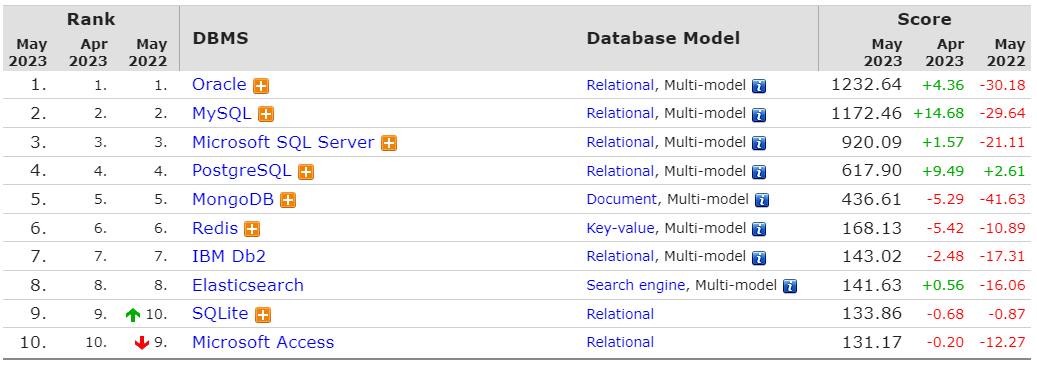
\includegraphics[width=14cm]{./assets/figures/MySQLPopularity.png}
        \caption{Popularité des différents SGBD dans le monde \label{MySQLPopularity.png}}
    \end{figure}
\end{center}
On voit également sur ce classement que les SGBD les deux permiers ont des scores assez similaires et ont tous deux de la marge sur leur concurrent qui occupe la troisième place. Je vais donc brièvement comparer Oracle avec MySQL.

\begin{center}
    \begin{figure}[H]%TODO : Changer la taille de cette image
        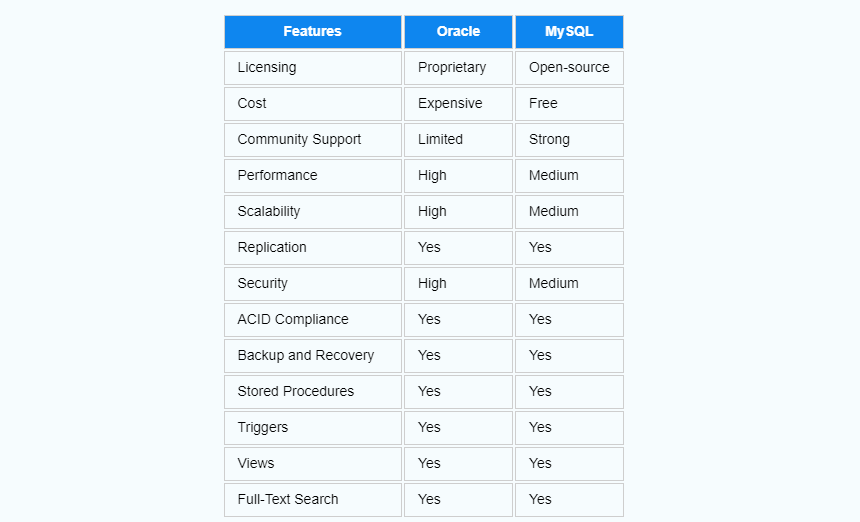
\includegraphics[width=\textwidth]{./assets/figures/OracleVsMySql.png}
        \caption{Comparaison entre Oracle et MySql \label{OracleVsMySql.png}}
    \end{figure}
\end{center}
Cependant comme montré dans l'article du site Integrate.io \cite{Integrate.io} les avantages sont minimes (des performances un peu meilleures et une sécuritée accrue). La licence Oracle étant cependant très onéreuse, ce dernier n'est pas un bon candidat dans le cadre de ce travail de Bachelor.

C'est pourquoi j'ai décidé de rester sur la version 8.0 de MySQL. Cependant, grâce au \emph{framework} Laravel il est extrêmement simple de changer de SGBD. En effet, il suffit de modifier le fichier de configuration. Si dans le futur, nous souhaitons pour une quelconque raison changer de SGBD, ce sera toujours possible et très facile.

\subsection{Laravel}
Laravel est un \emph{framework} \emph{open-source}, écrit en PHP, offrant une structure solide et élégante pour la création d'application et de site web. Le but principal de ce \emph{framework} est de simplifier la création et le développement d'application grâce à des fonctionnalités intégrées. Parmi ces fonctionnalités, on retrouve la gestion de routes, les sessions, l'authentification des utilisateurs ainsi que la gestion de la base de données.
Laravel fournit un ORM (\emph{Object Relational Mapping}), appelé Eloquent permettant de gérer toutes les interactions avec la base de données. Il permet également de choisir avec quel type de SGBD, nous souhaitons travailler et de changer ce dernier très rapidement grâce à des fichiers de configuration.
Il propose également un pattern architechtural très utilisé, le Modèle-Vue-Controller (MVC), que je vais rapidement expliquer.
\begin{center}
    \begin{figure}[H]%TODO : Changer la taille de cette image
        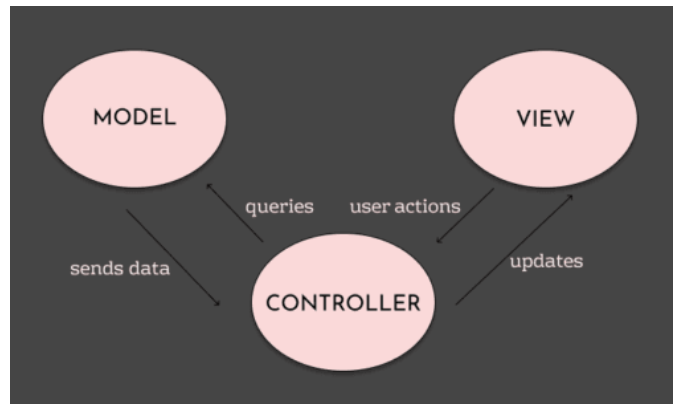
\includegraphics[width=\textwidth]{./assets/figures/MVCExplanation.png}
        \caption{Représentation du MVC \label{MVCExplanation.png}}
    \end{figure}
\end{center}

Sur cette capture, tirée du site Pusher \cite{MVC}, on peut voir les trois parties de ce système et comment elles interagissent.
\begin{itemize}
    \item Le Modèle est la partie responsable de la gestion des données ainsi que de la logique métier. C'est la seule partie du pattern qui interagit avec la base de données. Elle représente les structures de données, et fournit au \emph{Controller} des méthodes pour manipuler les données.
    \item La vue est la partie qui gère de l'interface utilisateur. Elle affiche les données et permet également de récupérer les informations saisies par l'utilisateur notamment au travers de formulaires.
    \item Le \emph{Controller} est la partie qui lie le Modèle et la Vue. Il réagit aux \emph{inputs} de l'utilisateur qui sont transmis par la Vue et va interroger, si nécessaire, le Modèle afin d'y mettre à jours ou récupérer des données. C'est également lui qui détermine quelle est la Vue à afficher à l'utilisateur. C'est le responsable de la logique de l'application.
\end{itemize}
Le MVC permet donc d'avoir une séparation distincte entre les différentes parties de notre application.

Un autre point fort de Laravel est sa gestion des \emph{middleware}. Un \emph{Middleware} est une sorte de filtre qui intervient lorsque les requêtes HTTP arrivent dans notre application. Cela permet notamment d'imposer qu'un utilisateur soit authentifié avant d'accéder à certaines ressources. Ils offrent donc un contrôle accru et centralisent la logique de certaines fonctionnalités.

Laravel est donc l'un des \emph{framework} les plus populaires, simple à prendre en main avec une documentation complète et mise à jour. Il est donc le candidat idéal pour ce projet. De plus, un changement de \emph{framework} imposerait une charge de travail supplémentaire bien trop conséquente.
Je vais donc utiliser la version 10 de Laravel.

\subsection{Vue.js}
Vue.js est un \emph{framework} JavaScript \emph{open-source}, populaire et polyvalent permettant de créer des interfaces utilisateur. Il est principalement utilisé pour le \emph{frontend} d'applications et peut facilement être ajouté à de gros projets. Il propose une approche basée sur les composants qui permettent de créer des portions de codes réutilisable. Grâce à une liaison bidirectionnelle entre les données et l'interface, Vue.js permet de synchroniser, en temps réel, les données entrées par l'utilisateur et leur affichage.

Ce qui permet à Vue.js d'être aussi performant est l'utilisation d'un \emph{DOM} virtuel. Le \emph{DOM (Document Object Model)} est une représentation hiérarchique d'un document HTML sous la forme d'un arbre. Il permet donc à des langages de programmation de modifier le style ou la forme de ce document. Cependant, à chaque changement, le navigateur va mettre à jour l'interface. Cela peut grandement impacter les performances si les modifications sont très fréquentes. C'est pourquoi Vue.js utilise un \emph{DOM} virtuel ou \emph{Virtual DOM}. Il s'agit d'une copie virtuelle stockée en mémoire du \emph{DOM} réel. Lors d'une mise à jour, les changements sont stockés dans le \emph{Virtual DOM}. Vue.js va ensuite comparer le \emph{Virtual DOM} avec le \emph{DOM} réel et n'appliquer que les changements nécessaires. Cela explique pourquoi ce \emph{framework} a des performances relativement élevées.

Pinia est le gestionnaire d'état conseillé pour la version 3 de Vue.js. Il permet de gérer l'état de l'application et de le partager entre les différents composants. Cet outil va nous être très utile au cours de ce projet.

Une autre fonctionnalité très importante de ce \emph{framework} est la capacité de créer des \emph{Singe Page Application} ou une application à page unique. Le concept derrière les SPA est que toute l'application est rendue sur une seule page. La SPA va initialement charger une page puis va dynamiquement changer son contenu en fonction des besoins et volontés de l'utilisateur. Cela permet une expérience utilisateur plus rapide et fluide qu'avec une application classique.

Les principaux concurrents du \emph{framework} Vue.js sont React et Angular. Selon un sondage réalisé par StackOverflow \cite{StackoverflowSurvey} en 2022, React est plus populaire que Vue.js et Angular.
\begin{center}
    \begin{figure}[H]%TODO : Changer la taille de cette image
        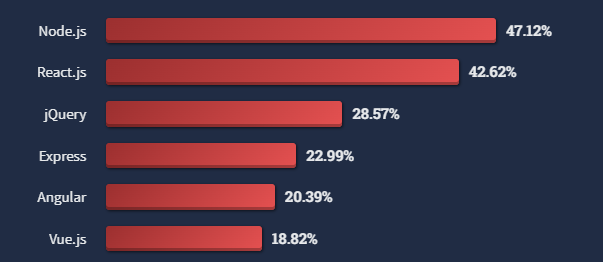
\includegraphics[width=\textwidth]{./assets/figures/VueVSReactVSAngular.png}
        \caption{Popularité des framework web \label{VueVSReactVSAngular.png}}
    \end{figure}
\end{center}

Comme Vue.js, React est un \emph{framework} javascript performant et dispose d'une communauté active. Il aurait été un bon choix de technologie pour ce projet, car plus utilisé dans l'industrie et disposant de plus d'utilisateurs.

Cependant, comme pour Laravel, un changement de \emph{framework} aurait imposé une charge de travail supplémentaire trop importante. De plus, Vue.js est plus simple à prendre en main et à utiliser que React. Il est donc mieux adapté à un projet de cette envergure. Je vais donc utiliser la version 3.0 de Vue.js.

\subsection{TailwindCSS}
TailwindCSS \cite{TailwindCSS} est un \emph{framework} CSS \emph{open-source} très simple à installer et utiliser. Il favorise la création rapide d'interfaces utilisateur personnalisées. Contrairement à son principal concurrent Bootstrap, TailwindCSS ne propose pas de composants prédéfinis. On y retrouve plutôt des classes utilitaires qui permettent de modifier rapidement le style d'un élément. Chaque classe est indépendante et ne représente qu'une fonctionnalité. Par exemple la classe "mb-4" permet d'ajouter une marge sur le bas d'un élément. Cela rend la personnalisation de l'interface utilisateur plus simple et plus rapide. On peut également créer ses propres classes utilitaires.

Un détail important de ce \emph{framework} est qu'il enlève tous les styles de base des navigateurs. Cela permet d'avoir une interface utilisateur cohérente sur tous les navigateurs.

Un autre point fort de ce TailwindCSS est sa communauté active. En effet, TailwindCSS dispose d'une documentation complète et de nombreux exemples.

Les raisons qui ont fait que j'ai choisi TailwindCSS sont sa simplicité d'utilisation, sa capacité de personnalisation. Bootstrap aurait été également un choix tout à fait valable. Cependant, pour avoir déjà travaillé avec ces deux \emph{framework}, j'ai une légère préférence pour TailwindCSS.

\subsection{Keycloak}
Keycloak \cite{Keycloak} est une solution \emph{open-source} de gestion d'identité et d'accès. Cela évite à notre application d'avoir à gérer les différents formulaires d'authentification, d'inscriptions ou de changement de mot de passe. Keycloak propose également une gestion des rôles et des permissions. Cela permet de définir des rôles pour les utilisateurs.

Dans le cadre de ce projet, tous les utilisateurs sont des membres de la HEIG-VD. Les deux choix que nous avions étaient d'utiliser Keycloak (le système de l'école) ou SWITCH edu-ID basé sur Shibboleth (actuellement utilisé dans le projet).

Le grand avantage de Keycloak est la maîtrise complète de l'outil par le service informatique de l'école. Cela permet une meilleure communication et entraide. De plus, Keycloak a déjà été utilisé sur plusieurs projets de l'école, donc sa mise en place sera simplifiée.
C'est pour ces raisons-là que j'ai décidé d'utiliser Keycloak.

\subsection{Github}
Github est une plateforme web de développement collaboratif basée sur Git. Elle facilite énormément la gestion de version de notre code source. De plus, elle favorise grandement la collaboration entre les différents développeurs. Github propose notamment des fonctionnalités de gestion de projet, permettant notamment des créer des tâches et de les assigner à des personnes. Ce qui aide à avoir une meilleure vue d'ensemble du projet.

Github permet également grâce à ses \emph{Github Actions} de créer des \emph{workflows CI/CD} qui permettent d'automatiser certaines tâches. Par exemple, on peut créer un \emph{workflow} qui va automatiquement lancer les tests unitaires à chaque modification du code qui sera poussé sur la plateforme. On peut également créer des \emph{Github Actions} qui vont déployer automatiquement notre application sur un serveur.

Github est la plateforme de gestion de version la plus populaire et la plus utilisée dans le monde. Selon les statistiques de l'article de Radix \cite{Radix}, Github aurait environ 56 millions d'utilisateurs contre 31 millions pour Gitlab. Avec son système de \emph{stars} et son côté social, Github est la plateforme idéale pour un projet open-source.

Toutes ces raisons font que Github est la plateforme de gestion de version choisie pour ce projet.
\newpage
\subsection{Récapitulatif des technologies}
Dans le tableau ci-dessous, vous pouvez trouver la liste de toutes les technologies qui sont utilisées dans le cadre de ce projet ainsi que leur version.
% Fais un tableau avec toutes les technologies utilisées dans le projet
\begin{table}[h]
    \begin{center}
        \caption{Technologies utilisées lors du projet \label{stack}}
        \begin{tabular}{|l|l|}
            \hline
            \textbf{Technologie} & \textbf{Version} \\
            \hline
            MySQL                & 8.0              \\
            \hline
            PHP                  & 8.2.6            \\
            \hline
            Composer             & 2.5.5            \\
            \hline
            Laravel              & 10               \\
            \hline
            Node                 & 18.15.0          \\
            \hline
            NPM                  & 9.5.0            \\
            \hline
            Vue.js               & 3                \\
            \hline
            Tailwind CSS         & 3.3.1            \\
            \hline
            WSL                  & 2                \\
            \hline
            Docker               & 20.10.22         \\
            \hline
            Ubuntu               & 22.04.2 LTS      \\
            \hline
            Keycloak local       & 21.1             \\
            \hline
            Github               & -                \\
            \hline
        \end{tabular}
    \end{center}
\end{table}

\chapter{Conception}




\chapter{Réalisation}
% Dans cette partie du rapport, je vais fournir les détails des actions effecutées ainsi que leurs justifications. J'exposerai également les défis rencontrés ainsi que leur solution.
% \section{Gestion de projet et Github}
% Bien qu'un \emph{repository} Github existe déjà, j'ai fait le choix de partir d'une base vierge. J'ai donc créé un nouveau \emph{repository} ainsi que deux nouveaux projets pour le \emph{frontend} et le \emph{backend}. Il s'agit donc d'un \emph{mono-repo}, c'est quand un seul \emph{repository} contient plusieurs projets distinct. En effet, il me semblait plus simple de partir d'une base nouvelle et de réutiliser les éléments du projet existant au fur et à mesure. De plus, cela me permet d'avoir une meilleure maîtrise du projet dans son entièreté.

% Une fois le travail terminé, il sera intéressant faire une \emph{Pull Request} sur le \emph{repository} de base afin de toujours avoir accès à toutes les versions et commit ce projet dans sa totalité.

% Ce \emph{repository} est accessible \href{https://github.com/Marinlestylo/h-quiz}{en cliquant ici}. Il est structuré de la manière suivante :
% \begin{itemize}
%     \item \textbf{Un dossier "api-backend"} : contient le code du de notre API.
%     \item \textbf{Un dossier "frontend"} : contient le code de l'interface utilisateur.
%     \item \textbf{Un fichier .gitignore} : Explicite tous les fichiers qui ne doivent pas être poussés sur GitHub.
%     \item \textbf{Un fichier README.md} : Explique les technologies et comment lancer le projet.
% \end{itemize}

% \subsection{User stories}
% GitHub offre un système d'issue qui permet de signaler qu'une fonctionnalité doit être réalisée. Cela permet de garder une trace de ce qui doit être fait et de les marquer comme finie, une fois implémentée. Cela permet également de voir l'avancement du projet. Vous pouvez trouver la liste de toutes les issues ouvertes \href{https://github.com/Marinlestylo/h-quiz/issues}{ici}. Il est important de noter qu'à ce stade du projet, les issues ne sont pas encore toutes écrites.

% GitHub nous offre également une vue d'ensemble de toutes ces issues. En effet, grâce à la fonctionnalité \emph{Projects}, nous pouvons créer des projets et y ajouter des issues. Avec la vue "tableau", nous avons une vue d'ensemble de toutes les issues et trois colonnes : \emph{To do}, \emph{In progress} et \emph{Done}. On peut donc savoir ce qui est en cours de réalisation. Ces fonctionnalités sont incroyablement utiles lorsqu'on travaille en équipe. Même si elles sont légèrement moins importantes quand on est seul sur un projet, cela nous permet de mesurer l'avancement du projet. C'est pour ces raisons que j'ai décidé d'utiliser ces fonctionnalités.

% \subsection{Branches et commits}
% Pour ce qui est de la gestion des branches, j'ai décidé de rester très simple et de n'utiliser que deux branches : \emph{main} et \emph{dev}. La branche \emph{main} est la branche principale. Elle doit être fonctionnelle à tout moment.

% La branche \emph{dev}, quant à elle, sera celle où je vais développer les fonctionnalités. Lorsque plusieurs fonctionnalités sont implémentées et sont entièrement fonctionnelles, je fusionne les branches dans \emph{main}.

% Je n'ai pas utilisé cette méthodologie de travail dès le début du projet. En effet, j'ai commencé par travailler directement sur la branche \emph{main} afin d'avoir une base solide pour le projet. Une fois que l'API, sa connexion avec Keycloak et les communications entre le \emph{frontend} et le \emph{backend} étaient fonctionnelles, j'ai créé la branche \emph{dev} et j'ai adopté cette méthodologie de travail.

% Pour ce qui est des \emph{commits}, je me base sur les \emph{Conventional Commits} \cite{ConventionalCommits}. Plus particulièrement, tous mes \emph{commits} sont écrits en anglais et sont tous préfixés par un type.

% Les types que j'utilise sont les suivants :
% \begin{itemize}
%     \item feat : Une nouvelle fonctionnalité a été ajoutée.
%     \item fix : Une erreur a été corrigée.
%     \item docs : La documentation a été modifiée.
%     \item chore : Création d'un projet ou d'un dossier.
%     \item refactor : Refactorisation d'une partie du code.
% \end{itemize}

% \section{Architecture de l'application}
% Comme brièvement mentionné dans la section précédente, l'application est divisée en deux parties bien distincte : le \emph{frontend} et le \emph{backend}. Le \emph{frontend} est l'interface utilisateur. C'est ce que l'utilisateur voit et avec quoi il interagit. Le \emph{backend} est une API REST. C'est cette API qui permet la communication avec la base de données et la gestion des utilisateurs.

% La communication entre le \emph{frontend} et le \emph{backend} se fait via des requêtes HTTP. Vous trouverez un schéma expliquant cette architecture ci-dessous.

% \fig[H, width=14cm]{Architecture de la plateforme}{Architecture.drawio}

% Voici également un digramme de séquence expliquant ce qu'il se passe lorsque l'utilisateur veut accéder à une page qui affiche tous les quiz auxquels il a accès.

% \fig[H, width=14cm]{Diagramme de séquence pour l'affichage de tous les quiz}{ArchitectureSequence.drawio}

% Il est important de noter que dans ce diagramme, il n'y a pas encore de notion d'authentification. Cette notion sera expliquée dans la section suivante.

% \section{Authentification}
% Dans cette sous-section, je vais expliquer comment a été gérée l'authentification via Keycloak.

% \subsection{Processus d'authentification}
% Pour implémenter l'authentification avec Keycloak, il y avait deux possibilités envisageables. La première option était de gérer la connexion avec Keycloak depuis le frontend. Cela implique que Keycloak retourne un \emph{token} d'authentification au \emph{frontend} et que ce dernier l'envoie à l'API à chaque requête. L'API vérifie ensuite la validité du \emph{token} auprès du serveur Keycloak et renvoie une réponse en conséquence. Cette approche est parfaitement viable et est utilisée dans d'autres projet de la HEIG-VD.

% Le point faible de cette approche est que le \emph{frontend} et le \emph{backend} doivent tous les deux travailler avec Keycloak. Cela implique que si on veut changer de fournisseur d'identité, il faut modifier les deux parties de l'application.
% C'est pour cette raison qu'une autre approche a été mise en place où uniquement le \emph{backend} travaille avec Keycloak.

% Le digramme de séquence qui suit explique de façon détaillée quel est le processus d'authentification. À noter que le processus de déconnexion est identique.
% \fig[H, width=14cm]{Digramme de séquence pour l'authentification d'un utilisateur}{connexionFlow.drawio}

% Même si c'est un processus assez long et complexe, il a le grand avantage que le \emph{frontend} n'a aucune connexion directe avec le serveur d'authentification. Si nous décidons dans le futur de changer de fournisseur d'identité, il ne faudra modifier que le \emph{backend}.

% \fig[H, width=14cm]{Accès à une ressource sans être authentifié}{forbidden401.drawio}

% Ce diagramme suivant illustre ce qu'il se passe lorsque l'utilisateur veut accéder à une page qui nécessite une connexion, mais que ce dernier n'est pas encore authentifié. Il reçoit une erreur 401 \emph{Unauthorized}. C'est l'erreur standard pour indiquer qu'une ressource est protégée et que l'utilisateur doit être authentifié pour y accéder. A noter qu'un mécanisme similaire sera mis en place si un utilisateur authentifié tente d'accéder à une ressource qui lui est interdite. Par exemple, un étudiant qui tenterait d'accéder à une ressource réservée aux enseignants. L'erreur qu'il recevrait serait ici une erreur 403 \emph{Forbidden}.

% \subsection{Keycloak}
% Pour l'implémentation, j'ai utilisé une librairie nommée Socialite Providers \cite{SocialiteProviders}. Cette librairie permet de gérer l'authentification avec Keycloak dans Laravel. Je me suis également inspiré du projet \emph{Fablab-name} \cite{FablabName} du Professeur Yves Chevallier qui utilise également cette librairie.

% En premier lieu, j'ai dû modifier le fichier \emph{app/providers/EventServiceProvider.php} afin d'y rajouter un \emph{event listener}.
% \begin{listing}[H]
%     \inputminted{php}{assets/code/serviceProviderkeycloak.php}
%     \caption{EventServiceProvider \label{serviceProviderkeycloak}}
% \end{listing}

% Suite à cela, il faut créer deux routes pour le \emph{login} et une pour le \emph{logout}. Ces routes sont définies dans le fichier \emph{routes/api.php}.

% \begin{listing}[H]
%     \inputminted{php}{assets/code/routeKeycloak.php}
%     \caption{Routes pour l'authentification Keycloak \label{routeKeycloak}}
% \end{listing}

% On peut voir que la route de déconnexion n'est accessible que par un utilisateur connecté pour éviter des erreurs.

% Finalement, j'ai créé un \emph{KeycloakController} qui s'occupe de gérer la logique de l'authentification. Ce fichier se trouve dans \emph{app/Http/Controllers/KeycloakController.php}.

% \begin{listing}[H]
%     \inputminted{php}{assets/code/keycloakController.php}
%     \caption{KeycloakController \label{keycloakController}}
% \end{listing}

% Dans ce \emph{Controller}, on va s'intéresser à trois méthodes :
% \begin{itemize}
%     \item \emph{redirect} : Cette méthode redirige l'utilisateur vers la page de login de Keycloak.
%     \item \emph{callback} : Cette méthode est appelée une fois que l'utilisateur s'est authentifié avec succès. Elle va ensuite créer ou modifier l'utilisateur dans la base de données. Finalement, elle va rediriger l'utilisateurs vers le \emph{frontend}.
%     \item \emph{logout} : Cette méthode va déconnecter l'utilisateur de Keycloak et le rediriger vers le \emph{frontend}.
% \end{itemize}

% La dernière modification est faite dans le fichier \emph{app/Http/Middleware/Authenticate.php}. C'est à cet endroit que l'on va vérifier si l'utilisateur est authentifié. Si ce n'est pas le cas, on retourne une erreur 401.

% \begin{listing}[H]
%     \inputminted{php}{assets/code/authenticate.php}
%     \caption{Renvoie de l'erreur 401 \label{authenticate}}
% \end{listing}


% \subsubsection{Modification de la base de données}
% Suite à cette implémentation, il m'a fallu faire des modifications dans la table \emph{users} de la base de données. En effet, les champs suivants ont été supprimés :
% \begin{itemize}
%     \item \emph{name} : Ce champ est une concaténation du nom et prénom de l'utilisateur. Il a donc été supprimé car ces informations sont redondantes.
%     \item \emph{password} : Ce champ n'existe tout simplement plus, car nous ne stockons pas le mot de passe du Keycloak.
%     \item \emph{api\_token} : Ce champ n'existe plus.
% \end{itemize}

% De plus, j'ai rajouté le champ \emph{keycloak\_id} qui contient l'identifiant unique de l'utilisateur dans Keycloak. Ce champ est utilisé pour vérifier si l'utilisateur existe déjà dans la base de données. Si c'est le cas, on met à jour les informations de l'utilisateur. Sinon, on crée un nouvel utilisateur.

% \section{Deployement}
% Même si ce n'est pas listé dans les objectifs de ce projet, il est important de déployer ce projet afin de vérifier que les fonctionnalités de dernier ne fonctionnent pas uniquement en local. Le projet est actuellement déployé à l'adresse suivante : \url{https://h-quiz.heig-vd.site/}. À noter que ce nom de domaine n'appartient pas à la HEIG-VD.

\chapter{Conclusion}
C'est la première fois que j'ai dû faire un vrai travail de \emph{refactor} sur un gros projet. Cela s'est avéré plus complexe que ce à quoi je m'attendais. En effet, chaque développeur à son propre fonctionnement et ses propres habitudes et c'est souvent ardu de bien comprendre ce qu'ils ont fait.

De plus, ce projet me permet mieux me rendre compte de l'importance capitale de la documentation lors de la reprise d'un projet existant. La documentation est souvent une partie du travail qui n'est pas du tout appréciée et qu'on a tendance de laisser de côté. J'espère que la personne qui reprendra ce projet aura plus de facilité que moi à le faire.

% TODO dire les fonctionnalités qui ont été perdues
% List de toutes les fonctionnalités

\vfil
\hspace{8cm}\makeatletter\@author\makeatother\par
\hspace{8cm}\begin{minipage}{5cm}
    %%if
    % Place pour signature numérique
    \printsignature
    %%fi
\end{minipage}

\clearpage
\printbibliography

\appendix
\appendixpage
\addappheadtotoc

%%if
\chapter{Installation du projet}

% Les annexes n'ont pas un contenu \underline{normatif} mais \underline{descriptif}. Tout contenu annexé ne doit pas être nécessaire à la bonne compréhension du travail.

% Les annexes contiennent généralement :

% \begin{itemize}
%     \item les dessins mécaniques (mises en plan);
%     \item les schémas électriques détaillés;
%     \item des photographies du projet;
%     \item des scripts et des extraits de code source;
%     \item des documents techniques \pex \emph{datasheet};
%     \item des développements mathématiques.
% \end{itemize}
% \section{Sous section}
% \lipsum[1]
%%fi

\let\cleardoublepage\clearpage
\backmatter

\label{glossaire}
\printnoidxglossary
\label{index}
\printindex

% Le colophon est le dernier élément d'un document qui contient des notes de l'auteur concernant la mise en page et l'édition du document : il est parfaitement optionnel.
% \input{colophon.tex}

\end{document}
